%%%%%%%%%%%%%%%%%%
%% Sample thesis using upnmthesis.cls, October 20, 2015.
%% by Lian Tze LIM (liantze@gmail.com)
%% http://liantze.penguinattack.org/latextypesetting.html#upnmthesis
%%
%% Possible options:
%% undergrad -- If you're writing an undergraduate thesis. There will then
%%              be no exam committee approval (even if you have specified
%%              examcommapproval), and the wordings of the supervisory
%%              committee approval will be different. Remember to specify
%%              your \faculty and \bachprogramme if using this option.
%% newtx --     Loads the newtxtext and newtxmath font packages if these
%%              packages are installed; they have nicer math fonts.
%%              Otherwise mathptmx will be loaded as default.
%% microtype -- Even nicer typographic output! Reduces chances of hyphenation
%%              but *sometimes* (though rare) may cause an endless loop as
%%              the typesetting engine tries to find an optimal line break.
%%%%%%%%%%%%%%%%%%
%\documentclass[undergrad,newtx,microtype]{upnmthesis}
\documentclass{upnmthesis}

%% Load any other packages you need here
\usepackage{graphicx}
\usepackage{lipsum}

%% Information about your thesis
\author{Muhammad Syafiq bin Md.~Akhir}
\title{\LaTeX{} Thesis Template for Universiti Pertahanan Nasional Malaysia}
\degree{Doctor of Philosophy}

%% If Bachelor programme, you'll need to uncomment and specify the following:
% \bachprogramme{Chemical Engineering}
% \faculty{Faculty of Engineering}

\submissionyear{2011}
\submissionmonth{October}
\vivadate{25 August 2011}

\begin{document}
%% Load myacronyms.tex, which contains your abbreviations etc
%!TEX ROOT=sample-thesis.tex

%% Format: \newacronym{label}{abbreviated form or symbol}{full form}
\newacronym{LI}{LI}{lexical item}
%% need to specify plural forms explicitly, otherwise will be
%% auto-genetared as "part of speechs"
\newacronym[firstplural={parts of speech (POS)},plural={POS}]%
{POS}{POS}{part of speech}
\newacronym{NLP}{NLP}{Natural Language Processing}
\newacronym{theta}{$\theta$}{temperature degree}
\newacronym{IR}{IR}{Information Retrieval}
\newacronym{WWW}{WWW}{World Wide Web}


\frontmatter

%% This will generate the cover page, a blank page, and then the title page
\makecoverandtitlepage

%% Dedication -- comment out if you don't need one
\dedication{To my parents.}

%% English and Malay abstracts in their respective files
\abstractfromfile{sample-abstract}
\msabstractfromfile{sample-msabstract}

%% Acknowledgements in a separate file
\begin{acknowledgements}
Thanks guys. I owe you many.
\end{acknowledgements}


%% Examination Committee Approval: Only required for graduate students.
%% Undegraduates may comment out this block.
\begin{examcommapproval}
  % Exam Committee Chairman
  \member[title=Professor, department={Faculty of Mathematics}, role={Chairman}]{Name of Chairperson, PhD}
  % Internal Examiner 1
  \member[title=Associate Professor, department={Faculty of Engineering}, role={Internal Examiner}]{Name of Examiner 1, PhD}
  % Internal Examiner 2
  \member[title={}, department={Faculty of Engineering}, role={Internal Examiner}]{Name of Examiner 2, PhD}
  % External Examiner
  \member[title=Associate Professor, department={School of Chemical Engineering}, institute={Imperial College}, role={External Examiner}]{Name of External, PhD}
\end{examcommapproval}

%% Supervisory Committee Approval
\begin{supervisoryapproval}
  % Supervisory Committee Chairman
  \member[title={Associate Professor}, role={Chairman}, department={Faculty of Engineering}]{Name of Chairperson, PhD}
  % Supervisory Committee Member 1
  \member[title={Ir.}, department={Faculty of Engineering}]{Name of Member 1, PhD}
  % Supervisory Committee Member 2
  \member[department={Faculty of Engineering}]{Name of Member 2, PhD}
\end{supervisoryapproval}


%% Declaration page -- remember to sign
\declarationpage


%% Content lists
{\clearpage\SingleSpacing
\tableofcontents*\clearpage
\listoftables\clearpage
\listoffigures\clearpage
%% Comment out the following line if
%% you have two or less appendices
% \listofappendices\clearpage
\printacronyms\clearpage
}

\mainmatter
%% Recommended to put chapters in separate files
%!TEX ROOT = sample-thesis.tex
\chapter{Introduction}

So this is the preamble at the beginning of the chapter. The purpose may be to introduce the themes of the chapter and main headings.

See how inter-paragraph spacing is larger. \lipsum[3]

\section{First Test and I need a really long title, please do oblige me won't you? Just a few more words and yes we're there}
\lipsum[1-2]

\begin{figure}[hbt!]\centering
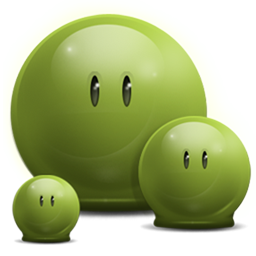
\includegraphics[width=.3\textwidth]{green}
\caption{First figure. OK?}
\end{figure}

\begin{figure}[hbt!]\centering
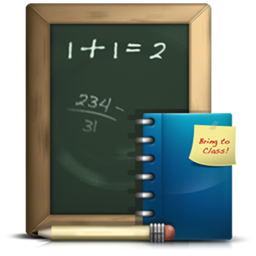
\includegraphics[width=.3\textwidth]{school}
\caption{Second figure. Now I need a long caption to test out how things look in the List of Figures. Is this long enough yet? Is it? Is it?}
\end{figure}


\begin{figure}[hbt!]
\centering
%
\begin{minipage}{0.3\textwidth}
\centering
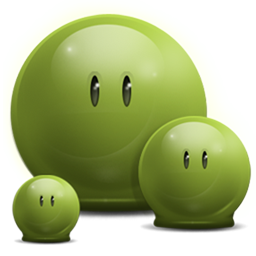
\includegraphics[width=\linewidth]{green}
\subcaption{The first subfigure}
\end{minipage}
%
\hspace{1cm}
%
\begin{minipage}{0.3\textwidth}
\centering
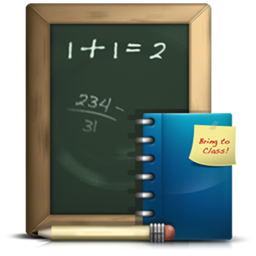
\includegraphics[width=\linewidth]{school}
\subcaption{The second subfigure}
\end{minipage}

\caption{An example with subfigures}
\end{figure}

\begin{subsecs}
\subsection{Second Test}
Their \cite{audibert:2004} requirements\footnote{See here, how weird, how to fill out an entire line. See here, how weird, how to fill out an entire line. See here, how weird, how to fill out an entire line. See here, how weird, how to fill out an entire line. See here, how weird, how to fill out an entire line. } are really amazing\footnote{don't you agree?} \cite{budanitsky:hirst:2006}.

Looks like everyting's working. Great. Let's talk about \glspl{LI} and \glspl{POS} in \gls{NLP}. I mention again \glspl{LI}. Oh I have a symbol too, it's \gls{theta}.

\subsection{This is another Subsection}

Remember that subsections need to be indented! 

\end{subsecs}

\section{Yeah}

And here's a long quotation, it should be an indented block and single-spaced:

\begin{quotation}
\lipsum[5]
\end{quotation}

Time for some maths, and later there's a table.

\begin{equation}
\left[M\frac{\partial }{\partial M}+\beta(g)\frac{\partial }{\partial g}+n\gamma\right] G^{(n)}(x_1,x_2,\ldots,x_n;M,g)=0
\end{equation}

\begin{table}[hbt!]
\caption{This is a table}
\centering
\begin{tabular}{ l c r }
\hline
Hey & How's it & Going?\\ \hline
Fine! & Just great. & See ya!\\
Fine! & Just great. & See ya!\\
\hline
\end{tabular}
\end{table}

\lipsum[7-12]
%!TEX ROOT = sample-thesis.tex
\chapter{Dummy Chapter}

Hello!!\index{furball}

\begin{figure}[hbt!]
\centering Test 3
\caption{Let's see. What have we got here?}
\end{figure}


%% Your .bib bibliography file (without .bib extension)
\bibliography{myrefs}

%% Recommended to put appendices in separate files
\begin{appendices}
%!TEX ROOT = sample-thesis.tex
\chapter{Manuals, Technical Specifications, Documentations, Example Scenarios}

%!TEX ROOT = sample-sample.tex
\chapter{Try}

\lipsum[1-2]

\end{appendices}

%% Your biodata, in biodata.tex
\begin{biodata}
Put your personal biodata as required here. \lipsum[1]
\end{biodata}

%% List of your own publications -- make sure you've
%% defined them in your bibliography .bib file.
\nociteown{Lim:2009,Bond:etal:WordNetBahasa:2014,Lim:etal:2014,Lim:etal:acl:lookup}
\bibliographyown{myrefs}

\end{document}